\documentclass[twoside, 12pt]{article}

\usepackage[sc]{mathpazo} % Use the Palatino font
\usepackage[T1]{fontenc} % Use 8-bit encoding that has 256 glyphs
\linespread{1.5} % Line spacing - Palatino needs more space between lines

%\usepackage[twoside,width=16cm,height=24cm,left=3cm]{geometry}
\usepackage[hmarginratio=1:1,top=20mm,width=20cm,height=23.7cm,columnsep=15pt]{geometry} % Document margins
\usepackage{multicol} % Used for the two-column layout of the document
\usepackage[hang, small,labelfont=bf,up,textfont=it,up]{caption} % Custom captions under/above floats in tables or figures
\usepackage{booktabs} % Horizontal rules in tables
\usepackage{float} % Required for tables and figures in the multi-column environment - they need to be placed in specific locations with the [H] (e.g. \begin{table}[H])
\usepackage{hyperref} % For hyperlinks in the PDF

%----------- Agregados para el caso de ustedes -------------------------------
\usepackage[spanish]{babel}% idioma castellano
\usepackage[utf8]{inputenc}% esto es para poder poner los tildes directamente. Puede que cambie de versión a versión de sistema operativos (más información en http://www.aq.upm.es/Departamentos/Fisica/agmartin/webpublico/latex/FAQ-CervanTeX/FAQ-CervanTeX-6.html )
\usepackage{graphicx} % para insertar figuras
\usepackage{subfigure} % para insertar figuras dentro de figuras
\usepackage{times} % plataforma
\usepackage{amsmath} % --para ecuaciones y algunos símbolos 
\usepackage{wrapfig,lipsum}
\usepackage{listings}
\usepackage{color}

\definecolor{dkgreen}{rgb}{0,0.6,0}
\definecolor{gray}{rgb}{0.5,0.5,0.5}
\definecolor{mauve}{rgb}{0.58,0,0.82}

\lstset{frame=tb,
	language=C++,
	aboveskip=3mm,
	belowskip=3mm,
	showstringspaces=false,
	columns=flexible,
	basicstyle={\small\ttfamily},
	numbers=none,
	numberstyle=\tiny\color{gray},
	keywordstyle=\color{blue},
	commentstyle=\color{dkgreen},
	stringstyle=\color{mauve},
	breaklines=true,
	breakatwhitespace=true,
	tabsize=3
}
% ---------------------- -----------------------------------------------------

\usepackage{lettrine} % The lettrine is the first enlarged letter at the beginning of the text
\usepackage{paralist} % Used for the compactitem environment which makes bullet points with less space between them
\usepackage[T1]{fontenc}					%para poder usar tildes sin problemas

\usepackage{mathrsfs}
% Abreviaturas
%\newcommand\RR{\mathbb{R}}

\graphicspath{{Imagenes/}}

\begin{document}

\begin{center}
{\fontsize{20pt}{10pt}\textbf{Implementación de potenciales y compiladores}}
\end{center}

El objetivo fue generar un método para implementar el cálculo de las fuerzas totales en un sistema de $N_{part}$ partículas para un potencial dado. Esta función \texttt{forces} debía ser tan general como fuese posible para así evitar problemas a la hora de cambiar el potencial. Implementamos estas funciones en C y, posteriormente, comparamos su velocidad de ejecución para distintas optimizaciones del compilador: \texttt{O0}, \texttt{O1}, \texttt{O2}, \texttt{O3} y \texttt{Ofast}. 

La opción \texttt{O0} es la opción por default en la que no hay optimizaciones mientras que \texttt{O1} es la opción con optimizaciones elementales. Por otro lado, la optimización \texttt{O2} realiza todas las optimizaciones que no envuelven \textit{space-speed tradeoff} (mayor uso de memoria en pos de aumentar la velocidad). La opción \texttt{O3}, en cambio, si realiza este tipo de optimizaciones como el inlineado de funciones y la vectorización de ciclos. Finalmente, la opción \texttt{Ofast} hace todo esto junto optimizaciones que no son \textit{standard-compliant} como \texttt{-ffast-math}; librería con funciones matemáticas implementadas para tener una mayor velocidad pero no necesariamente arrojar resultados con la exactitud apropiada. 

\section{Implementaciones}
Con esto en mente, planteamos 9 posibles implementaciones de la función \texttt{forces} combinando distintos rasgos. En todos los casos (excepto el primero), \texttt{forces} llamaba otras funciones para ejecutar el cálculo de la fuerza (\texttt{pair\_force}) o energía (\texttt{pair\_energ}) de interacción entre 2 partículas. 

Los rasgos que fuimos modificando son: 

\begin{quote}
\begin{description}
\item[Precalculo:] El pre-cálculo o no de parámetros relevantes para la interacción tanto en la energía como en la fuerza de 2 partículas

\item[Auxiliares:] Separar el cálculo auxiliar en 2 funciones distintas \texttt{pair\_force} y \texttt{pair\_energ} o tener una única función \texttt{pair\_energ\_force}

\item[Modulo:] Que la función auxiliar que calcula la fuerza de interacción devuelva el vector completo (con sus 3 componentes) o solo el módulo.
\end{description}
\end{quote}

Comparamos todas estas funciones con una función \texttt{forces1} sin funciones auxiliares que, en principio, sería la más veloz. Así, fue posible evaluar que tanta velocidad de ejecución se perdía en pos de la encapsulación del potencial. 

\subsection{Estabilización del tiempo de ejecución}

Preliminarmente, buscamos el valor de $N_{part}$ a partir del cual el tiempo de ejecución resultaba $\tau\sim N_{part}^2$ dado que la cantidad de interacciones que \texttt{forces} calculaba es $N_{part}(N_{part}-1)/2\sim N_{part}^2$, bajo la hipótesis de que el tiempo de cómputo de la interacción entre 2 partículas es independiente de sus posiciones. Para asegurar esto último, evitamos la aplicación de un radio de corte $r_c$ para el potencial (en este caso Morse) que lo anule $\forall r\geq r_c$.

Esto lo hicimos calculando el tiempo que tomaba computar $N_{iter}$ veces las fuerzas de un sistema de $N_{part}$ partículas. Los resultados se muestran en la \textbf{Figura \ref{fig:TvsNpart}} y permiten extrapolar que para simulaciones cuya duraci\'on sea mayor a $1ms$ o $N_{part}\geq200$, el comportamiento es cuadr\'atico en $N_{part}$.

\begin{figure}[h]
	\centering
	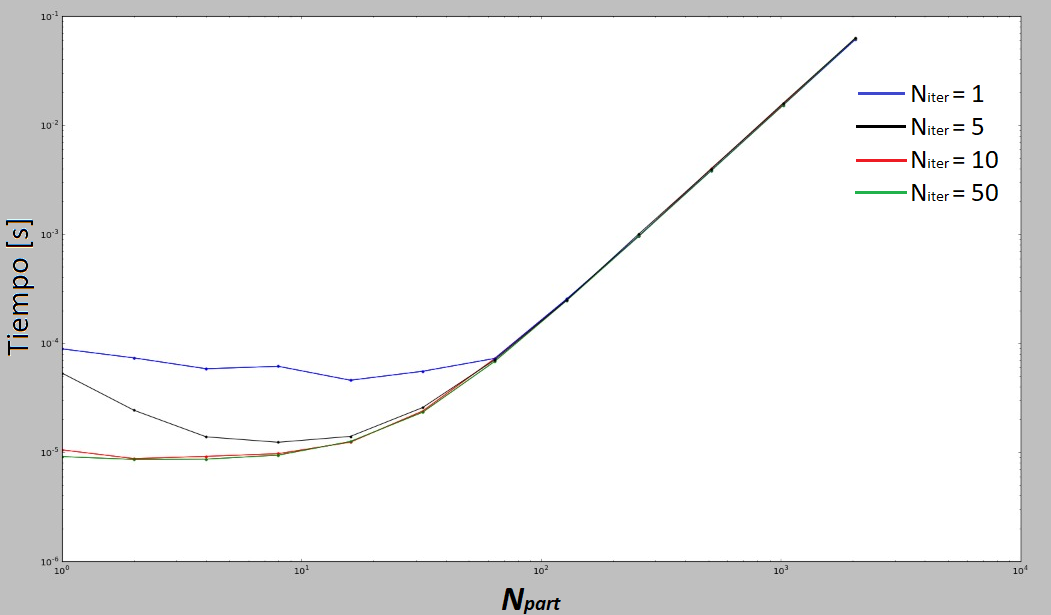
\includegraphics[width=0.65\columnwidth]{Estabilizacion_Npart.png}
	\caption{Tiempo de ejecución de $N_{iter}$ \texttt{forces} para $N_{part}$ partículas. Para $N_{part}>200$ el tiempo ya es polinómico (cuadrático) para todo $N_{iter}$. Esto se condice con simulaciones cuya duraci\'on supera $1ms$}
	\label{fig:TvsNpart}
\end{figure}

\subsection{Comparación: Potencial de Morse}

El primer potencial que implementamos fue el de Morse

\[ V_{M} (r) = D\left[1-e^{-\alpha (r-r_{eq})}\right]^2\]

Realizamos 9 implementaciones del mismo, destacando la implementaci\'on 1 por ser la m\'as directa y las funciones 5 y 9 por su mayor portabilidad y devolviendo el módulo de fuerza.

\begin{quote}
\begin{description}
\item[1] Sin funciones auxiliares.
\item[5] Dos funciones, con parámetros precalculados, devuelve modulo de fuerza.
\item[9] Dos funciones, sin parámetros precalculados, devuelve modulo de fuerza (encapsula totalmente el potencial).
\end{description}
\end{quote}

\begin{multicols}{3}
\begin{lstlisting}
float forces1(...){
	...
	for(i=0;i<N;i++){
		for(j=i+1;j<N;j++){
			...
			calculo 
			de fuerza
			...
			calculo 
			de energia
			...
		}	
	}
}
\end{lstlisting}
\columnbreak
\begin{lstlisting}
float forces5(...){
	...
	for(i=0;i<N;i++){
		for(j=i+1;j<N;j++){
			...
			precalculo de parametros
			...
			pair_force(params,..)
			pair_energ(params,..)
		}	
		...
	}
	...
}

float pair_force(params,..){
...
}

float pair_energ(params,..){
...
}
\end{lstlisting}

\columnbreak
\begin{lstlisting}
float forces9(...){
	...
	for(i=0;i<N;i++){
		for(j=i+1;j<N;j++){
			pair_force(...)
			pair_energ(...)
		}	
		...
	}
	...
}

float pair_force(..){
	calculo de 
	parametros
	...
}

float pair_energ(..){
	calculo de 
	parametros
	...
}

\end{lstlisting}

\end{multicols}


Esta portabilidad permite usar las 2 funciones auxiliares como \textit{test} directamente desde \texttt{Python} y aprovechan que el vector dirección de la fuerza es independiente del potencial. Las demás funciones son:

\begin{quote}
\begin{description}
\item[2 y 3] Única función auxiliar \texttt{pair\_energ\_force} con y sin parámetros precalculados.
\item[4] Como \texttt{forces5} pero devolviendo el vector completo
\item[6] Como \texttt{forces9} pero con algunos parámetros precalculados (no todos).
\item[7 y 8] Versiones de \texttt{forces6} y \texttt{forces9} con una única función auxiliar \texttt{pair\_energ\_force}.
\end{description}
\end{quote}

Compilando con los distintos optimizaciones \texttt{O} corrimos las simulaciones para sistemas con $N_{part}=216$. Calculamos el tiempo por par de interacci\'on mediante 
\[ \tau_{par}=\frac{2\tau}{N_{part}(N_{part}-1)} =\frac{\tau}{23220} \]
donde $\tau$ era el tiempo total de duraci\'on de la simulaci\'on, obtenido mediante estad\'istica sobre $1000$ corridas. Los resultados pueden apreciarse en la \textbf{Figura \ref{fig:CompTodas}}.

\begin{figure}[h]
	\centering
	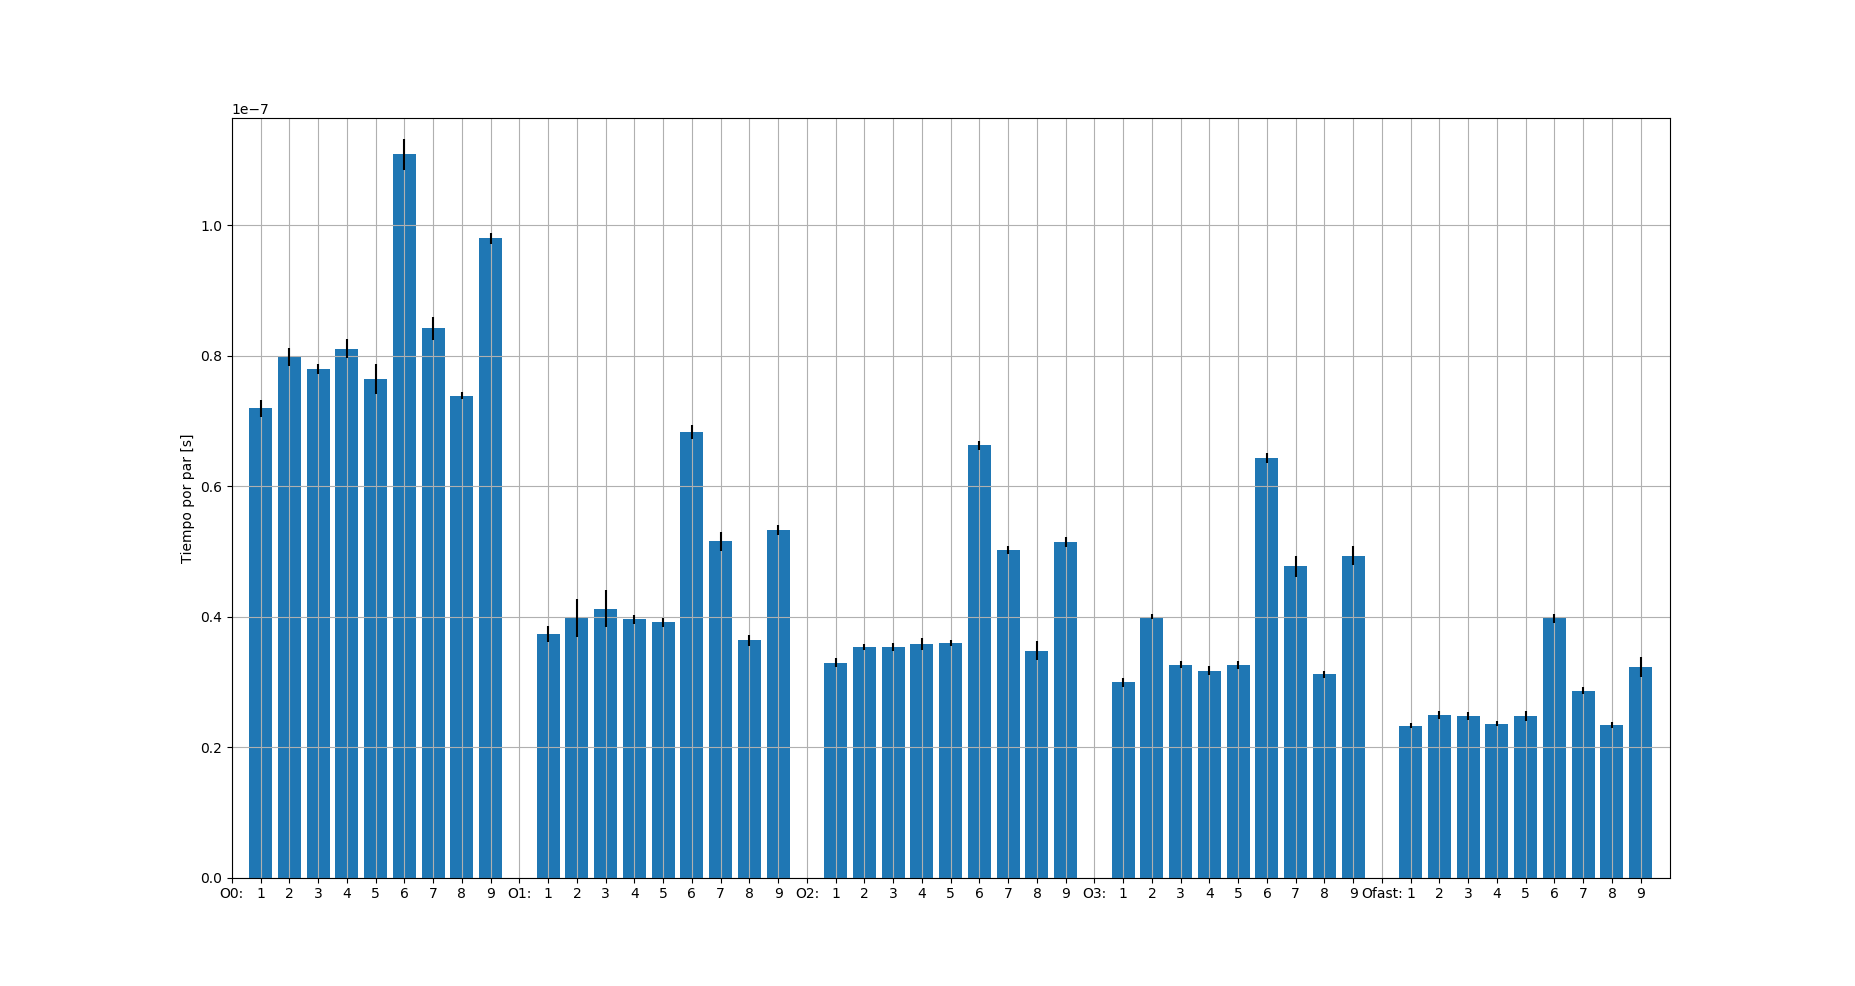
\includegraphics[trim = 40mm 20mm 40mm 20mm, clip, width=\columnwidth]{Comp_tiempos_morse_todos.png}
	\caption{Comparación de tiempos para las distintas implementaciones del potencial de morse. La tendencia decreciente de \texttt{O0} a \texttt{Ofast} es clara, excepto excepciones puntuales de \texttt{O2} a \texttt{O3}.}
	\label{fig:CompTodas}
\end{figure}

En general, puede verse una tendencia decreciente a medida que se pasa de \texttt{O0} a \texttt{Ofast}, lo cual resulta esperable. Sin embargo, algunas excepciones notables se dan en el paso de \texttt{O2} a \texttt{O3}.

De mayor inter\'es es notar que el compilador \texttt{Ofast} logra que las implementaciones 2, 3, 4 y 5 tengan diferencias menores al $5\%$ entre si y respecto de la implementaci\'on 1, volvi\'endolas virtualmente equivalentes.  Por tanto, estas 4 implementaciones bien pueden ser reemplazadas unicamente por 5, que resulta m\'as portable como dijimos previamente.

Adem\'as, viendo que las implementaciones 6 y 7 tienen tiempos comparables a 9, resulta razonable reemplazarlas por 9. En el caso de \texttt{forces9} es importante aclarar que, al no tener ningún parámetro precalculado, la encapsulación del potencial es completa. Desde el punto de vista de la ingeniería de software \texttt{forces9} sería la óptima. 

Por lo tanto,aislamos las funciones \texttt{forces1}, \texttt{forces5} y \texttt{forces9} para cuantificar la pérdida de velocidad en pos de la portabilidad (encapsulación del potencial) y se volvieron a correr las simulaciones, obteniendo los resultados de la \textbf{Figura \ref{fig:CompEsp}}

\begin{figure}[h]
	\centering
	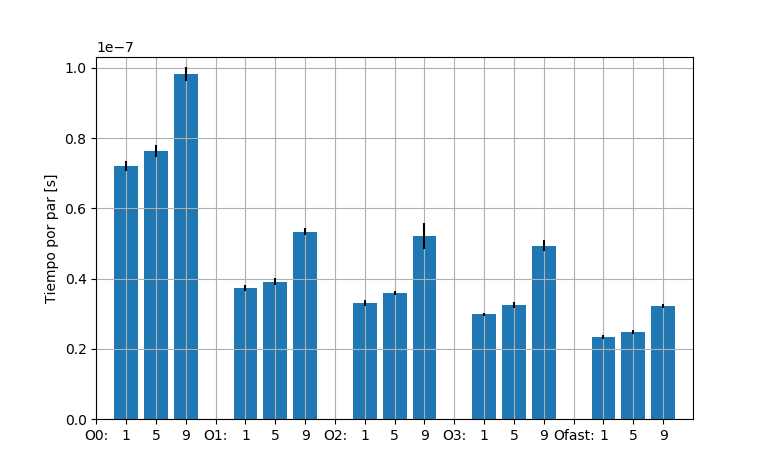
\includegraphics[trim = 10mm 5mm 10mm 5mm, clip, width=0.6\columnwidth]{Comp_tiempos_morse.png}
	\caption{Comparaci\'on de las implementaciones de mayor portabilidad (5 y 9) contra la implementaci\'on directa 1. Aunque 1 parece equivalente a 5, difiere con 9 en $\sim 40\%$}
	\label{fig:CompEsp}
\end{figure}

Como observamos previamente, la implementaci\'on 5 resulta equivalente a la 1 para todos los \texttt{O} (excepto \texttt{O0}). Sin embargo, la implementaci\'on 9 resulta notoriamente m\'as lenta, con una diferencia relativa respecto a 1 que crece a medida que pasamos de \texttt{O0} a \texttt{Ofast} (donde alcanza un $\sim40\%$). Esto \'ultimo puede deberse a que la separaci\'on en 2 funciones obliga a calcular la funcion \texttt{exp} 2  veces, lo cual no ocurre en la implementacion 1 (es directa) ni en la 5 (la exponencial se pasa como par\'ametro precalculado). Dado que la exponencial no es una funci\'on elemental, sus tiempos elevados de calculo pueden causar esta discrepancia.

\subsection{Comparación: Potencial de Lennard-Jones}

Con el objetivo de confirmar que la abismal diferencia entre la implementaci\'on 9 y la 1 se debe al c\'alculo de \texttt{exp}, realizamos un an\'alisis similar al anterior para el potencial de Lennard-Jones \[ V_{LJ} (r) =  4\varepsilon \left[ \left(\frac{r}{\sigma}\right)^{12} -\left(\frac{r}{\sigma}\right)^{6} \right] \]

Este potencial se calcula utilizando solamente operaciones algebraicas elementales (multiplicaci\'on, suma, resta y divisi\'on). Realizamos las siguientes implementaciones, an\'alogas a 1, 5 y 9 en el caso del potencial de Morse
	
\begin{quote}
\begin{description}
\item[1] Sin funciones auxiliares.
\item[2] Dos funciones, con parámetros precalculados, devuelve modulo de fuerza.
\item[3] Dos funciones, sin parámetros precalculados, devuelve modulo de fuerza (encapsula totalmente el potencial).
\end{description}
\end{quote}

An\'alogamente, hicimos corridas con cada optimización \texttt{O}, promediando los tiempos con $1000$ corridas. Los resultados se encuentran en la \textbf{Figura \ref{fig:CompEsp_LJ}}, donde puede verse el gran salto entre \texttt{O0} y \texttt{O1}, con sus sucesivos saltos de menor orden. En particular, entre \texttt{O3} y \texttt{Ofast} no hay ninguna mejora de velocidad. Sin embargo, sigue manteniendose la abismal diferencia entre la implementaci\'on 9 y la 1 de un $40\%$.

\begin{figure}[h]
	\centering
	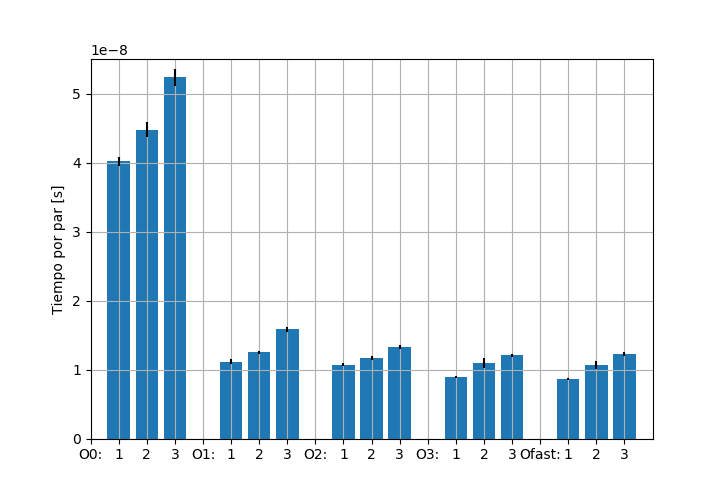
\includegraphics[trim = 10mm 5mm 10mm 5mm, clip, width=0.6\columnwidth]{Comp_tiempos_LJ.png}
	\caption{Comparaci\'on de las implementaciones de mayor portabilidad contra la implementaci\'on directa 1. A diferencia del caso de Morse, la implementaci\'on 2 y 3 resultan notoriamente m\'as lentas que la 1.}
	\label{fig:CompEsp_LJ}
\end{figure}

En particular, comparando las \textbf{Figuras \ref{fig:CompEsp}} y \textbf{\ref{fig:CompEsp_LJ}} puede verse que el c\'alculo de LJ resulta el doble de r\'apido que el de Morse. Esto permitir\'ia pensar que aproximadamente la mitad del tiempo de c\'omputo se invierte en calcular \texttt{exp}, hecho que oculta la diferencia real entre la implementaci\'on 1 y 5 de Morse, que ahora pasa a ser $\sim 20\%$. 

\section{Inlineado de funciones}

Los resultados previos parecen apuntar al hecho de que los tiempos de simulaci\'on se ven afectados por el hecho de que la funci\'on \texttt{forces} llame funciones auxiliares \texttt{pair\_force} y \texttt{pair\_energ}. Este tiempo puede reducirse dr\'asticamente utilizando \textit{function inlining}, que en \texttt{C} se reduce a agregar el sufijo \texttt{inline} delante de la declaraci\'on de la funci\'on. Este inlining fuerza al compilador a copiar la funci\'on dentro del cuerpo del c\'odigo en lugar de llamarla durante su ejecución. 

Dado que las funciones estan ahora dentro del cuerpo del c\'odigo, resulta razonable pensar que los optimizaciones \texttt{O} ser\'an capaces de optimizar la funci\'on \texttt{forces} en conjunto con \texttt{pair\_force} y \texttt{pair\_energ}. Por lo tanto, en el caso del potencial de Lennard-Jones ser\'ia factible hacer el c\'alculo de los par\'ametros precalculables dentro de \texttt{pair\_force} y \texttt{pair\_energ}, con la esperanza de que los optimizaciones lo noten y efectivamente los precalculen fuera de ellas.

Hicimos entonces una versi\'on equivalente a \texttt{forces3} de LJ con estos últimos cambios y se la corri\'o bajo los mismos par\'ametros de antes, obteniendo los resultados de la \textbf{Figura \ref{fig:CompEsp_LJ_inline}}.

\begin{figure}[h]
	\centering
	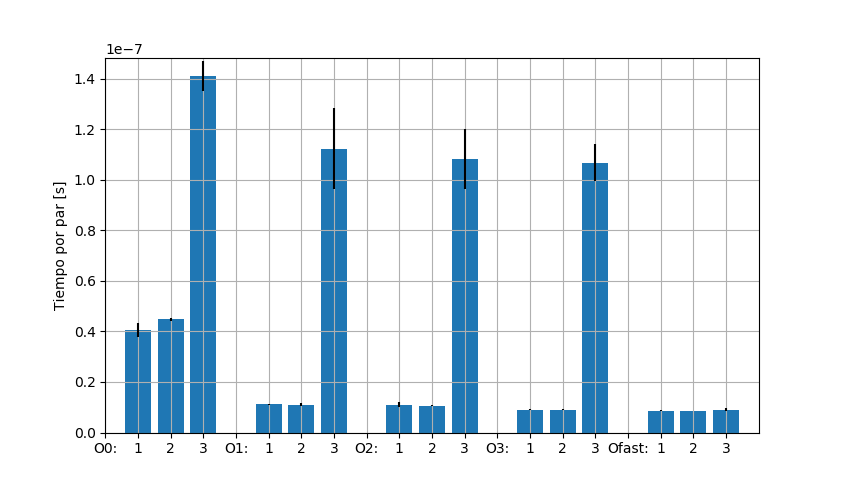
\includegraphics[trim = 10mm 5mm 10mm 5mm, clip, width=0.6\columnwidth]{Comp_tiempos_LJ_inline.png}
	\caption{Comparaci\'on de las implementaciones de Lennard-Jones de mayor portabilidad contra la implementaci\'on directa 1 utilizando inlining. Solo la optimización \texttt{Ofast} logra volver las implementaciones 1 y 9 comparables; es el \'unico que realiza los precalculos de variables fuera de \texttt{pair\_force} y \texttt{pair\_energ}}
	\label{fig:CompEsp_LJ_inline}
\end{figure}

Los resultados son muy alentadores, dado que las 3 implementaciones resultan indistinguibles dentro del error bajo la optimizaci\'on \texttt{Ofast}. En particular, puede verse como esta modificaci\'on resulta terriblemente perjudicial para los los dem\'as optimizaciones, que claramente no realizan el precalculo. 

Finalmente, realizando un trabajo complemente an\'alogo con el potencial de Morse, obtuvimos los resultados de la \textbf{Figura \ref{fig:CompEsp_morse_inline}}. Nuevamente, en el caso de \texttt{Ofast} las 3 implementaciones resultan indistinguibles. Sin embargo, puede verse como el c\'alculo de \texttt{exp} nuevamente enmascara las abismales diferencias entre la implementaci\'on 1 y 9 para las dem\'as optimizaciones.

\begin{figure}[h]
	\centering
	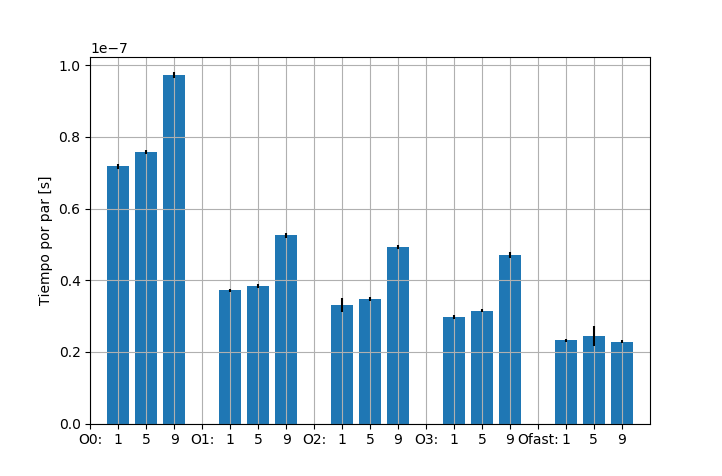
\includegraphics[trim = 10mm 5mm 10mm 5mm, clip, width=0.6\columnwidth]{Comp_tiempos_morse_inline.png}
	\caption{Comparaci\'on de las implementaciones de Morse de mayor portabilidad contra la implementaci\'on directa 1 utilizando inlining. A diferencia del caso de LJ, la diferencia resulta menos notoria, enmascarada por el c\'alculo de \texttt{exp}}
	\label{fig:CompEsp_morse_inline}
\end{figure}

\section{Conclusiones}

Sin m\'as preambulos, resulta inmediato elegir la implementaci\'on de \texttt{forces} con dos funciones auxiliares \texttt{pair\_force} y \texttt{pair\_energ} inlineadas sin parametros precalculados, que devuelvan el modulo de la fuerza. Esta opci\'on ya era la \'optima del punto de vista de ingenier\'ia de software y, gracias al previo an\'alisis, resulta equivalente en t\'erminos de velocidad.

Con esto tenemos una encapsulación total del potencial, permitiendo la implementaci\'on de un \texttt{forces} como marco general que funciona para cualquier par de funciones auxiliares \texttt{pair\_force} y \texttt{pair\_energ}. Estas funciones auxiliares son las que introducir\'an efectivamente el potencial dentro del c\'alculo; para cambiar el potencial basta cambiar estas funciones auxiliares.

\textbf{MÁS DISCUSIÓN, MAS IDEAS: LO QUE SIENTA QUE APRENDI}

\end{document}
